\documentclass[10pt]{article}
\usepackage[total={170mm,230mm}]{geometry}

\usepackage{cmap}
\usepackage{hyphsubst}
\usepackage[utf8]{inputenc}
\usepackage[T1]{fontenc}
\usepackage[russian]{babel}

\usepackage{graphicx}
\usepackage{xcolor}
\usepackage{amssymb}
\usepackage{amsfonts}
\usepackage{amsmath}
\usepackage{amsthm}
\usepackage{physics}
\usepackage{wrapfig}
\usepackage{cancel}
\usepackage{pdfpages}
\usepackage{hyperref}
% \usepackage{bibtex}

\title{Домашнее задание №2. Метод ортогональных коллокаций}
\author{Александр Козлов}
\date{\today}

\begin{document}

\maketitle

\section*{Формулировка задания}

Дан гамильтониан одномерной квантово-механической системы с потенциалом в виде гауссовой ямы
\begin{equation}
    H = - \dv[2]{}{x} + V_0\, e^{-x^2},
\end{equation}
где $V_0 < 0$. Требуется сделать следующее.

\begin{enumerate}
    \item Найти константы связи $V_0$, при которых в системе возникает одно, два и три связанных состояния.

    \item Исследовать зависимость вычислительных затрат от размера сетки.

    \item Исследовать зависимость погрешности энергий состояний от размера сетки и границ бокса.
\end{enumerate}

Задания следует выполнять методом коллокации с разложением по набору функций в пространстве кубических сплайнов $S_{3,2}$.

\section{Дискретизация задачи и численное решение}

Рассматриваемое уравнение Шрёдингера (УШ) имеет вид
\begin{equation}
    -\dv[2]{\psi}{x} + V_0\, e^{-x^2}\, \psi  = E\, \psi
    \label{eq:SE}
\end{equation}
или
\begin{equation}
    \dv[2]{\psi}{x}  + (E - V_0\, e^{-x^2})\, \psi  = 0.
\end{equation}
Стоит заметить, что такое уравнение соответствует обычному одномерному УШ при $\hbar=1$ и $m=1/2$.

Прежде всего зададим равномерную сетку
\begin{equation}
    x_0 = -R,\; x_1 = x_0 + \delta,\; x_2 = x_0 + 2\delta,\; \ldots,\; x_k = x_0 + k\delta,\; \ldots,\; x_M = x_0 + M \delta = R
\end{equation}
с шагом $\delta = 2R/M$, где $M$~---~целое положительное число, а $R$~---~положительное действительное число.

Решать уравнение будем методом, основанным на разложении волновой функции по некоторому набору функций $S_l(x)$
\begin{equation}
    \psi(x) = \sum\limits_{l} f_l S_l(x).
    \label{eq:decomp}
\end{equation}

\subsection{Набор функций}



Для каждой $k$-ой точки сетки определена пара функций $\Phi_k$ и $\Psi_k$, каждая из которых в свою очередь определяется как кусочно заданная функция на интервале $x\in(x_{k-1},\; x_{k+1})$ следующим образом:
\begin{equation}
    \begin{split}
        \Phi_{k}(x) =
        \begin{cases}
         -\dfrac{2}{\delta^3}(x-x_{k})^3 - \dfrac{3}{\delta^2}(x-x_{k})^2 + 1, & x\le x_k\\
         &\quad\\
         \dfrac{2}{\delta^3}(x-x_{k})^3 - \dfrac{3}{\delta^2}(x-x_{k})^2 + 1, & x>x_k
        \end{cases},\\
        \quad\\
        \Psi_{k}(x) =
        \begin{cases}
         \dfrac{1}{\delta^2}(x-x_{k})^3 + \dfrac{2}{\delta}(x-x_{k})^2 + (x-x_{k}), & x\le x_k\\
         &\quad\\
         \dfrac{1}{\delta^2}(x-x_{k})^3 - \dfrac{2}{\delta}(x-x_{k})^2 + (x-x_{k}), & x>x_k
        \end{cases}.
    \end{split}
\end{equation}
Полезны выражения для вторых производных этих функций, поэтому выпишем их
\begin{equation}
    \begin{split}\Phi_{k}^{\prime\prime}(x) =
        \begin{cases}
         -\dfrac{12}{\delta^3}(x-x_{k}) - \dfrac{6}{\delta^2}, & x\le x_k\\
         &\quad\\
         \dfrac{12}{\delta^3}(x-x_{k}) - \dfrac{6}{\delta^2}, & x>x_k
        \end{cases},\\
        \quad\\
        \Psi_{k}^{\prime\prime}(x) =
        \begin{cases}
         \dfrac{6}{\delta^2}(x-x_{k}) + \dfrac{4}{\delta}, & x\le x_k\\
         &\quad\\
         \dfrac{6}{\delta^2}(x-x_{k}) - \dfrac{4}{\delta}, & x>x_k
        \end{cases}.
    \end{split}
\end{equation}
Из функций $\Psi$ и $\Phi$ нужно собирать набор, по которому будем раскладывать нашу волновую функцию. Набор функций можно ввести следующим образом:
\begin{equation}
    S_l(x) =
    \begin{cases}
        \alpha_1 \Psi_0(x) + \alpha_2 \Phi_0(x), &l=1;\\
        \beta_1 \Psi_M(x) + \beta_2 \Phi_M(x), &l=2M;\\
         \Phi_{(l-1)/2}(x), &{l\,\textrm{mod}\,2 = 1\textrm{ и }l\ne 1};\\
        \Psi_{l/2}(x), &{l\,\textrm{mod}\,2 = 0\textrm{ и }l\ne 2M}
    \end{cases}
    ,\quad l = \overline{1, 2M}.
\end{equation}
Параметры $\alpha$ и $\beta$ выбираются на основе поставленного граничного условия. Для определённости поставим нулевое граничное условие
\begin{equation}
    \psi(x_0) = \psi(x_M) = 0,
\end{equation}
тогда параметры $\alpha$ и $\beta$ можно выбрать такими:
\begin{equation}
    \alpha_2=\beta_2=0,\quad \alpha_1=\beta_1=1.
\end{equation}

В итоге получим
\begin{equation}
    S_l(x) =
    \begin{cases}
        \Psi_0(x), &l=1;\\
        \Psi_M(x), &l=2M;\\
         \Phi_{(l-1)/2}(x), &{l\,\textrm{mod}\,2 = 1\textrm{ и }l\ne 1};\\
        \Psi_{l/2}(x), &{l\,\textrm{mod}\,2 = 0\textrm{ и }l\ne 2M}
    \end{cases}
    ,\quad l = \overline{1, 2M}.
\end{equation}

\subsection{Точки коллокации}

В качестве точек коллокации будут использованы нули второго полинома Лежанра на отрезке $\qty[-1,\;1]$, отображённые с этого отрезка на отрезки сетки $\qty[x_{k-1},\;x_{k}],\; k=\overline{1,M}$. Кратко точки коллокации определить можно следующим образом:
\begin{equation}
    x^{(c)}_t =
    \begin{cases}
        x_{(t-1)/2} + \dfrac{\delta}{2} \qty(1 - \dfrac{1}{\sqrt{3}}), &{t\,\textrm{mod}\,2 = 1};\\
        x_{t/2} - \dfrac{\delta}{2} \qty(1 - \dfrac{1}{\sqrt{3}}), &{t\,\textrm{mod}\,2 = 0}
    \end{cases}
    ,\quad t = \overline{1, 2M}.
\end{equation}

\subsection{Проекция уравнения Шрёдингера на дельта-функции}

Подставляем разложение волновой функции по кубическим сплайнам \eqref{eq:decomp} в уравнения Шрёдингера \eqref{eq:SE} и проецируем полученное уравнение на дельта-функции $\delta(x-x^{(c)}_t)$, приходим к соотношению
\begin{equation}
    \sum\limits_{l=1}^{2M} f_{l}
    \mel**{\delta(x-x^{(c)}_t)}{H-E}{S_{l}(x)}=0,\quad t=\overline{1,2M}.
\end{equation}
Функции $S_l(x)$ мы выбрали локализованными, это позволяет заметно сократить число слагаемых в уравнении, так как дельта-функция с центром в точке $x^{(c)}\in\qty[x_{k-1},\;x_{k}]$ даёт ненулевые интегралы лишь для тех $S_l(x)$, которые отличны от нуля на интервале $\qty[x_{k-1},\;x_{k}]$. Однако, для записи этого вывода требуется учитывать чётность $t$. Нетрудно получить, что для нечетного индекса $t$ выживают слагаемые с индексом $l=t-1,\;t,\;t+1,\;t+2$, а для четного $t$ выживают слагаемые с индексом $l=t-2,\;t-1,\;t,\;t+1$.

Задача сводится к обобщённой задаче на собственные значения/собственные вектора, которую можно представить в виде:
\begin{equation}
 \begin{split}
  \qty(\hat A - E \hat B) \vb{f} = 0,\\
  \vb{f} = (f_1,\, \ldots,\, f_{2M})^\textrm{T},\\
  A_{l,t} = \mel**{\delta(x-x^{(c)}_t)}{H}{S_{l}(x)},\\
  B_{l,t} = \braket{\delta(x-x^{(c)}_t)}{S_{l}(x)}.
 \end{split}
\end{equation}
Если матрица $\hat B$ обратима, то можно смести задачу к стандартной задче на собственные значения / собственные вектора, домножив слева на матрицу  $\hat B^{-1}$, тогда получаем уравнение
\begin{equation}
 \qty(\hat B^{-1} \hat A - E \hat I) \vb{f} = 0.
\end{equation}

\section{Количество связанных состояний в зависимости от константы связи}

При размере сетки $M=300$ и ширине бокса $R=20$ была получена зависимость числа связанных состояний от параметра связи, показанная на Рис. \ref{fig:n_vs_v0}.
\begin{figure}[htbp]
    \centering
    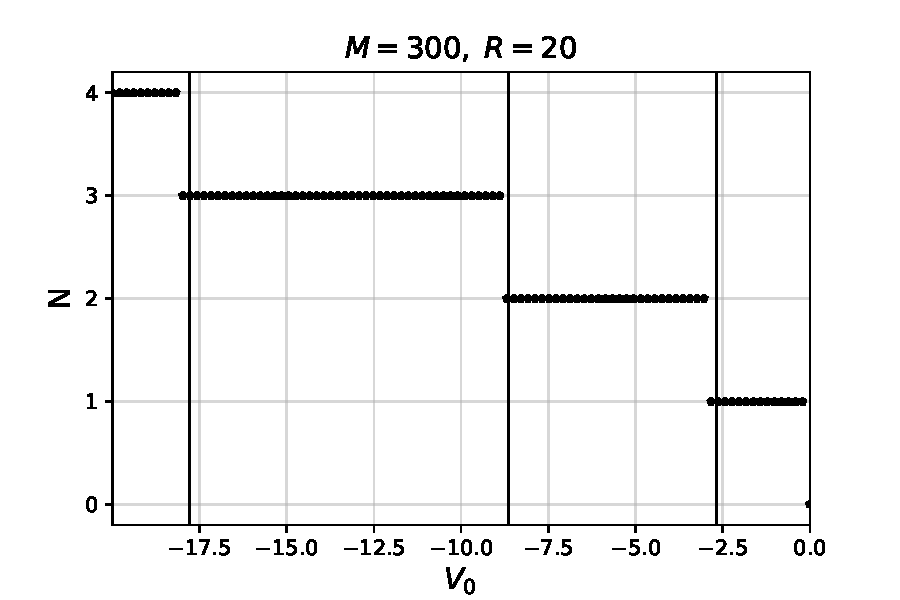
\includegraphics[width=0.75\textwidth]{../figures/num_eigen_vs_v0}
    \caption{Количество связанных состояний $N$ в зависимости от константы связи $V_0$ при размере сетки $M=300$ и ширине бокса $R=20$. Вертикальными линиями отмечены границы, адаптированные из работы \cite{article}.}
    \label{fig:n_vs_v0}
\end{figure}
Для оценки правильности полученных результатов обратимся к работе \cite{article}, где рассматривается уравнение, похожее на нашее за исключением того, что $v_0$ в статье соответсует $-V_0/2$ у нас. Если учесть разницу в обозначениях, то можно вынести из данной работы, что одно связанное состояние существует при $0 < \abs{V_0} < 2.684$, два связанных состояния --- при $2.684 < \abs{V_0} < 8.650$, три состояния --- при $8.650 < \abs{V_0} < 17.796$. Видно, что значения константы связи, при которых происходят скачки числа связанных состояний, примерно совпадают.


\section{Зависимость времени работы программы от размера сетки}

Определим, как долго работает программа при различных значениях параметра $M$ --- размера сетки. Для определённости фиксируем прочие параметры задачи, например, положим их следующими: $V_0 = -1.0$ и $R=20$. Результаты продемонстрированы на Рис. \ref{fig:T_vs_M}.
\begin{figure}[htbp]
    \centering
    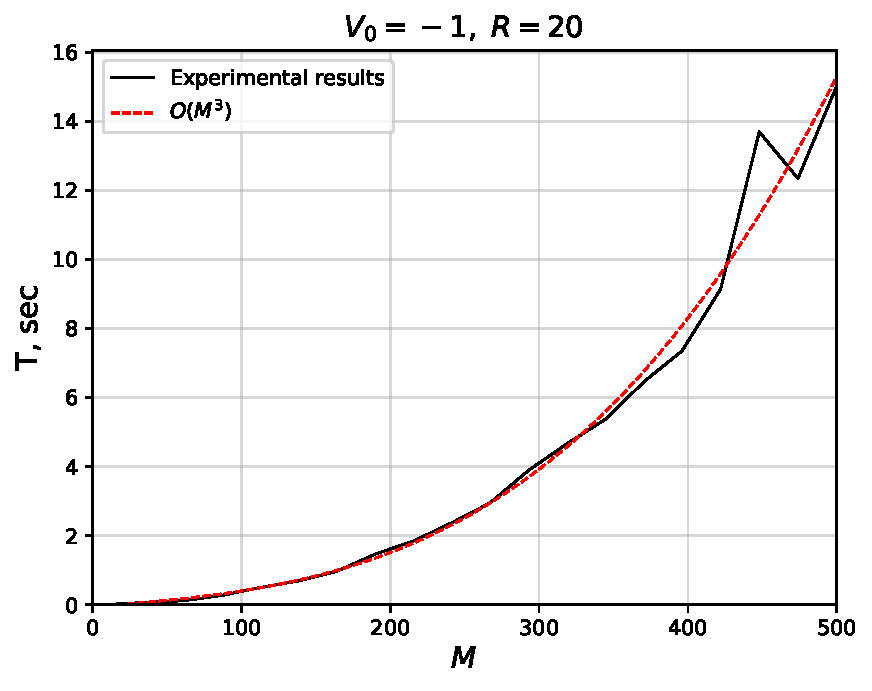
\includegraphics[width=0.75\textwidth]{../figures/T_vs_M}
    \caption{Время работы программы в секундах в зависимости от размера сетки $M$ при $V_0 = -1.0$ и $R=20$ (черная линия) и аппроксимация такой зависимости параболой (красная пунктирная линия).}
    \label{fig:T_vs_M}
\end{figure}

\section{Зависимость ошибки определения уровней энергии от размера сетки и размера бокса}

Рассмотрим случай $\abs{V_0}=1$. Для такого случая вариационный метод даёт оценку $E_1 = -0.335$. В качестве наиболее точного значения энергии взято эталонное значение энергии основного состояния из первого домашнего задания $E_0 = -0.3539907385825565$. На Рис. \ref{fig:abserr} представлены результаты расчётов.
\begin{figure}[htbp]
    \centering
    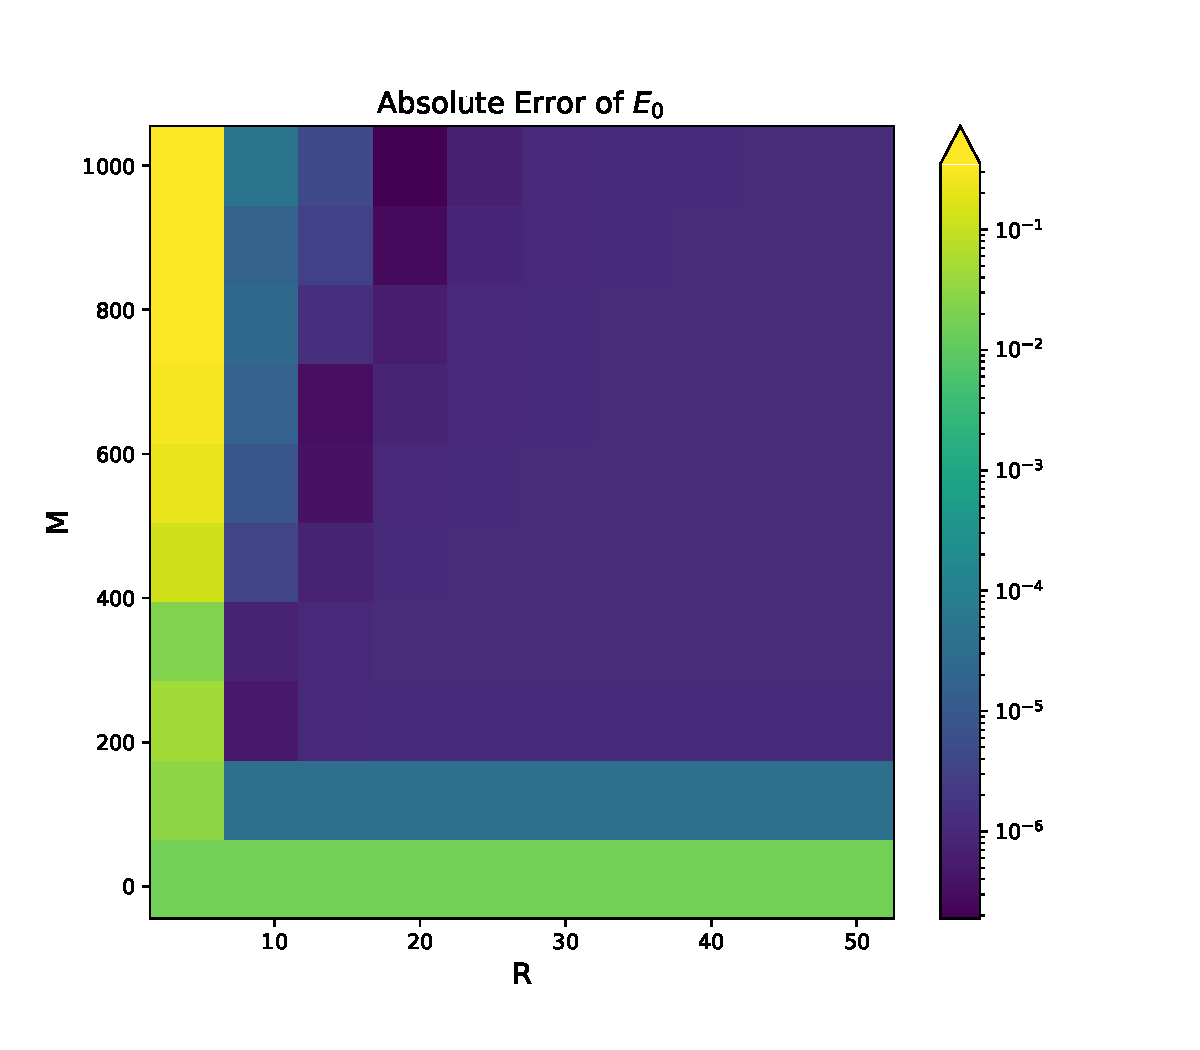
\includegraphics[width=0.75\textwidth]{../figures/abserr}
    \caption{Абсолютная ошибка вычисления энергии основного состояния при различных размерах сетки $M$ и бокса $R$ для случая $\abs{V_0}=1$.}
    \label{fig:abserr}
\end{figure}



\begin{thebibliography}{10}
    \bibitem{article}
    Fernández, Francisco.
    \newblock Quantum Gaussian wells and barriers.
    \newblock {\em Amer. \ J. \ Phys.}, 79:752--754, 2011.
\end{thebibliography}
\end{document}
